\documentclass[12pt, oneside,a4paper]{report}
\usepackage[czech, english]{babel}
\usepackage[T1]{fontenc} % pouzije EC fonty
\usepackage[utf8]{inputenc}

\usepackage{graphicx}
\usepackage{wrapfig}        % pro obtékání textu kolem obrázk? a tabulek 

\newcommand\TypeOfWork{Bakalářská práce}  \typeout{Bakalarska prace}

\newcommand\StudProgram{Geodézie a Kartografie, strukturovaný, Bakalářský}
\newcommand\StudBranch{Geoinformatika}

\newcommand\WorkTitle{Vector-to-vector conflation}
\newcommand\FirstandFamilyName{Tereza Fiedlerová}
\newcommand\Supervisor{Ing. Martin Landa}

\usepackage[
pdftitle={\WorkTitle},
pdfauthor={\FirstandFamilyName},
bookmarks=true,
colorlinks=true,
breaklinks=true,
urlcolor=red,
citecolor=blue,
linkcolor=blue,
unicode=true,
]{hyperref}

\begin{document}

\selectlanguage{czech}

\iflanguage{czech}{
	 \typeout{************************************************}
	 \typeout{Zvoleny jazyk: cestina}
	 \typeout{Typ prace: \TypeOfWork}
	 \typeout{Studijni program: \StudProgram}
	 \typeout{Obor: \StudBranch}
	 \typeout{Jmeno: \FirstandFamilyName}
	 \typeout{Nazev prace: \WorkTitle}
	 \typeout{Vedouci prace: \Supervisor}
	 \typeout{***************************************************}
	 \newcommand\Department{Katedra mapování a kartografie}
	 \newcommand\Faculty{Fakulta stavební}
	 \newcommand\University{České vysoké učení technické v Praze}
	 \newcommand\labelSupervisor{Vedoucí práce}
	 \newcommand\labelStudProgram{Studijní program}
	 \newcommand\labelStudBranch{Obor}
}

%%%%%%%%%%%%%%%%%%%%%%%%%%    Titulni stranka / Title page 

%\coverpagestarts

%\begin{titlepage}
% F
%\end{titlepage}


%%%%%%%%%%%%%%%%%%%%%%%%%%%   Prohlaseni / Declaration 

%\declaration{V Doksích dne \today}

%%%%%%%%%%%%%%%%%%%%%%%%%%%%    Abstract 

%\abstractpage
%\begin{abstract}
%This bachelor's project deals with the problem of ...

%\vglue60mm

%\noindent{\Huge \textbf{Abstrakt}}
%\vskip 2.75\baselineskip

%\noindent
%Tato bakalářská práce se zabývá problémem ...
%\end{abstract}

%%%%%%%%%%%%%%%%%%%%%%%%%%%%%%%%  Obsah / Table of Contents 

%\tableofcontents


%%%%%%%%%%%%%%%%%%%%%%%%%%%%%%%  Seznam obrazku / List of Figures 

%\listoffigures


%%%%%%%%%%%%%%%%%%%%%%%%%%%%%%%  Seznam tabulek / List of Tables

%\listoftables


%**************************************************************

%\mainbodystarts

\normalfont
%\parskip=0.2\baselineskip plus 0.2\baselineskip minus 0.1\baselineskip

%**************************************************************


\cleardoublepage\chapter{Úvod}
\label{1-uvod}


Tato práce se zabývá 'vector-to-vector conflation'.



\section{Seznam zkratek} % asi přesunout do jiné kapitoly
\label{zkratky}

\begin{tabular}{ll}
API & rozhraní pro programování aplikací (\textit{Application Programming Interface})\\ % nebo raději aplikační rozhraní?
DT & Delaunayho triangulace (\textit{Delaunay Triangulation})\\
GEOS & Geometry Engine, Open Source \\
GIS & Geografický informační systém (\textit{Geographic Information System}) \\
GPL & GNU General Public License \\
IDE & Vývojové prostředí (\textit{Integrated Development Environment})\\
JCS & Java Conflation Suite \\
JOSM & Java OpenStreetMap Editor \\
JTS & Java Topology Suite \\
LGPL & GNU Lesser General Public License \\
OGC & Open Geospatial Consorcium \\
OSGeo & Open Source Geospatial Foundation \\
QGIS & Quantum GIS \\
SQL & Structured Query Language \\
TIN & Nepravidelná trojúhelníková síť (\textit{Triangulated Irregular Network}) \\
WKT & Well Known Text \\  % možná zmizí !!
\end{tabular}


\cleardoublepage\chapter{Conflation}
\label{2-conflation}

Cílem této kapitoly je přiblížit čtenáři pojem sloučení vektorových map
(\textit{conflation}). Kro\-mě definice samotného pojmu kapitola popisuje 
i~klasifikaci sjednocování map a~obecný postup při této úloze. Hned zpočátku
bych však ráda upozornila na~to, že v~angličtině používaný pojem 
\textit{conflation} nemá žádný oficiální český ekvivalent, proto je v~některých
případech uveden v~originálním znění, aby nemohlo dojít k~špatnému výkladu 
textu.

\section{Definice pojmu \textit{conflation}}
\label{definice}

Pojem \textit{conflation} byl poprvé v~souvislosti s~kartografií a~\zk{GIS}
použit manželkou Jamese Corbetta, matematika působícího v~US~Census Bureau.
Termín pochází z~latinského \textit{con flare}, což znamená \uv{rozdmýchávat}
nebo doslovněji \uv{foukat dohromady}. Ještě před tím, než se toto slovo 
objevilo v~digitální kartografii, používalo se pro popis spojování dvou 
rukopisů do~třetí verze, která je kombinací těchto předchozích.

\textit{Conflation} lze do~češtiny přeložit jako slučování či spojování map. 
Překlad tohoto pojmu však není vždy jasný, jelikož se jím označuje více různých 
úloh, procesů či činností. Někdy bývá tento výraz zaměňován s~anglickými 
termíny \textit{map matching, map merging, rubber sheeting} atd., které obecně
označují činnosti spadající do této oblasti. Jelikož žádná oficiální česká
definice tohoto pojmu neexistuje, jsou zde uvedeny překlady definic z~různých 
zahraničních zdrojů. 

\begin{itemize}

  \item Sada činností, které vzájemně zarovnávají prvky dvou geografických
    datových vrstev a~následně převádí atributy jedné vrstvy do~druhé.
    
    (Wiki.GIS.com - The GIS Encyclopedia Glossary, 
    \url{http://wiki.gis.com/wiki/index.php/GIS\_Glossary/C},
    citováno 30.~4.~2013)

  \item \textit{Feature conflation} je proces kombinování geografických 
    informací z~překrývajících se zdrojových dat, který zachovává přesnost 
    dat, minimalizuje nadbytečná data a~předchází konfliktům v~datech.
    Potřeba \textit{conflation} vyvstává s~nutností aktualizace dat kvůli
    přesnosti či chybějícím prvkům/atributům pomocí novějších datových zdrojů
    zahrnujících překrývající se území.
    \textit{Conflation of geospatial data} (geoprostorových dat) je spojení
    či sladění dvou různých prostorových datasetů zahrnujících stejné území.
     
    (Shekhar, Xiong: Encyclopedia of GIS \cite[][s.~129]{gisencyclopedia})

  \item Proces sjednocení dvou rozdílných datasetů.
    
    (Blasby, Davis, Kim, Ramsey: GIS Conflation Using Open Source Tools 
    \cite[][s.~2]{opensourceconflation})

 \item \textit{Conflation} je proces, jehož cílem je geometricky upravit 
    (posunem, transformací) di\-gitální data zobrazující stejné území 
    (obvykle pořízená v~jiném čase) tak, aby byla vzájemně geograficky 
    \uv{korektní} a~vzájemně se překrývaly.
    
    (HUIC Data Services, \url{http://huic.com/HUIC/job/right/conflation.htm}, 
     citováno 30.~4.~2013)

  \item Schopnost kombinovat data z~různých zdrojů do~jednoho společného
    datasetu je jedním ze~základních problémů v~\zk{GIS}. Tato úloha je
    ve~vědecké literatuře označována jako \textit{conflation} prostorových
    dat.
   
    (Freitas, Afonso: Distributed Vector Based Spatial Data Conflation 
    Services \cite[][s.~23]{freitas})

  \item Soubor funkcí a~procedur, které zarovnávají prvky jednoho \zk{GIS} 
    souboru k~prvkům jiného a~následně převádí atributy mezi~těmito vrstvami.
    Zarovnání předchází převodu atributů a~je nejčestěji prováděno 
    \textit{rubber-sheeting} operacemi.
   
    (Prince George's County - GIS Glossary,
    \url{http://www.princegeorgescountymd.gov/Government/AgencyIndex/OITC/GIS/glossary.asp#C},
    citováno 30.~4.~2013)

  \item Proces sladění poloh odpovídajících si prvků v~různých datových 
    vrstvách. Funkce pro spojení map (\textit{conflation}) provádějí toto 
    sladění tak, aby se odpovídající si prvky přesně překrývaly. 
    
    (Geographic Information Nova Scotia - Standards Manual,
    \url{http://www.gov.ns.ca/snsmr/land/standards/post/manual/appedxa1.asp#C},
     citováno 30.~4.~2013)

\end{itemize}

\section{Historie}
\label{historie}

Až do 80.~let 20.~století bylo pořízení digitálních dat velmi drahé, a~proto 
se často nestávalo, že by nějaká firma vlastnila více mapových souborů jediného 
území. S~vývojem počítačů a~digitálních technologií se však tato data stávala 
stále do\-stupnějšími a~náhle vyvstala potřeba kombinovat data o~jednom území 
z~více zdrojů a~provádění aktualizace těchto dat. 

Jako první se k~takovému množství dat dostaly pochopitelně různé vládní 
instituce. Ačkoli první článek o~problematice spojování geografických dat 
z~více zdrojů vyšel už v~roce 1981 (\textit{M. White: The~Theory of~Geographical
Data Conflation}), k~opravdovému rozvoji došlo až po~roce 1985. V~té době 
totiž vznikl projekt, jehož cílem bylo propojení mapových souborů organizací
US~Census Bureau a~US~Geological Society. Vzhledem k~množství dat bylo nutné
celý proces co nejvíce auto\-matizovat. Použitý algoritmus, jehož hlavním autorem
je Alan Saalfeld, byl založen na~nalezení odpovídajících si prvků a~následné 
transformaci dat. 

S~narůstající dostupností dat a~zveřejněním této myšlenky přibývalo i~menších 
firem zabývajících se problémem kombinace mapových souborů z~různých zdrojů.

Zatímco před dvaceti lety se datasety slučovaly pouze na~základě geometric\-kých 
a~topologických vlastností, dnes stále větší roli hrají i~atributy jednotlivých 
prvků, které mohou práci velmi usnadnit. Nejnovějším přístupem je pak zjišťování 
sémantické podobnosti, která je založena na~porovnávání atributů, datových 
struktur a~vzájemných vztahů.


\section{Klasifikace \textit{conflation}}
\label{klasifikace}

\subsection{Dle území zobrazovaného vstupními vrstvami}
\label{dle-uzemi}
\nopagebreak
\begin{enumerate}
  \item \textbf{Horizontální} 
    \subitem Za~\textit{horizontal conflation} se označují procesy, které 
	zpracovávají data ze~vzájemně sousedících území. Cílem je získat 
	mapové soubory, jejichž hranice na~sebe dokonale navazují, a~to pokud 
	možno bez~ztráty přesnosti.
  \item \textbf{Vertikální} \nopagebreak
    \subitem Při~\textit{vertical conflation} obsahují vstupní data překrývající
	se území. Jde tedy o~dva či více souborů zobrazujících jediné území nebo
	alespoň jeho část. Může se jednat o~dvě verze té samé mapy nebo 
	o~dva datasety s~nějakými společnými prvky a~vlastnostmi. Výsledkem 
	celého procesu je jediný dataset, jehož přesnost není horší než přesnost
	původních dat a~obsahuje informace z~obou zdrojů. Jde tedy o~vylepšenou, 
	obsahově bohatší mapu s~odpovídající přesností. 
\end{enumerate}

\subsection{Dle typu vstupních vrstev}
\label{dle-vstupu}

\begin{enumerate}
  \item \textbf{Imagery to imagery, Raster to raster}
    \subitem Jedná se o~případ, kdy je úkolem na~sebe napasovat dva rastrové 
      mapové soubory. Nejčastěji jde o~ortofoto a~naskenovanou analogovou mapu
      daného území. Pomocí této úlohy můžeme například porovnat starou analogovou
      mapu se~současným stavem reprezentovaným právě leteckým snímkem. 
      Řešení tohoto problému vyžaduje poměrně složité techniky pro~nalezení 
      odpovídajících si objektů. Velmi důležitým faktorem je kvalita a~rozlišení
      vstupních dat.
  \item \textbf{Vector to imagery, vector to raster}
    \subitem Kombinace vektorových a~rastrových dat stejného území se využívá 
      často ke~zpřesnění vektorových dat jejich napasováním na~ortofoto. Hlavní
      náplní této oblasti je vývoj algoritmů umožňujících následující 
      \cite{gisencyclopedia}: 
	      \begin{enumerate}
	       \item Detekce charakteristických hran rastrového obrazu a~jejich 
		  porovnání s~vektorovými daty.
	       \item Využití vektorových dat k~identifikaci hran v~rastru - tzv. 
		  \textit{Snakes algorithm}.
	       \item Užití stereo obrazu, výškových dat a~dalších znalostí
		  pro~porovnání vektorových a~rastrových dat. 
	       \item Využití prostorových informací a~jiných vlastností mapy 
		  (jako např. barev) k~roz\-poznání odpovídajících si prvků.
	      \end{enumerate}
  \item \textbf{Vector to vector} \nopagebreak
    \subitem Případem sloučení dvou vektorových datasetů se zabývá tato práce. 
	Jednou ze~spe\-cifických a~velmi častých aplikací je navázání silničních 
	sítí, dále aktualizace digitál\-ních map aj. Existuje mnoho různých algoritmů
	pro~slučování vektorových dat, přičemž základní přístupy k~řešení problému 
	jsou následující \cite{gisencyclopedia}: 
	      \begin{enumerate}
	       \item Sloučení dat za~pomoci algoritmů, které pracují na~základě 
		  porovnávání geome\-trických vlastností prvků.
	       \item Algoritmy, které berou v~potaz podobnost tvarů prvků a~zároveň
		  podobnost jejich atributů.
	       \item Spojení vektorových dat s~neznámým souřadnicovým systémem 
		  na~základě rozmí\-stění významných bodových prvků (např. křižovatky 
		  cest).
	      \end{enumerate}

\end{enumerate}

  \begin{figure}[H]
    \centering
      \small
      \input{./pictures/klasifikace.pdf_tex}
      \caption{Klasifikace \textit{conflation} dle vstupních vrstev}
      \label{fig:classification}
  \end{figure}

\section{Obecný postup}
\label{postup}

Obecný postup při~slučování vektorových map z~více zdrojů se skládá z~několika
kroků, které jsou uvedeny níže. Jako u~většiny podobných operací je třeba 
nejdříve provést přípravu dat a~následně data zpracovat a~upravit.

\begin{enumerate}
  \item \textbf{Předzpracování dat}
    \subitem Tento krok slouží k~zajištění kompatibility vstupních dat tak, 
      aby bylo možné je porovnávat. Obvykle spočívá v~převedení vstupních 
      datasetů do~stejného souřadnico\-vé\-ho systému, zajištění stejných 
      základních jednotek a~dalších měnších úpravách. 
  \item \textbf{Kontrola kvality dat a~topologické správnosti vrstev}
    \subitem Zde se kontroluje vnitřní konzistence dat každé vstupní vrstvy.
      V~tomto případě záleží především na~požadavcích zvoleného algoritmu 
      pro~sloučení map. Může jít na\-pří\-klad o~odstranění topologických chyb 
      v~dané vrstvě jako jsou nežádoucí drobné překryty či mezery 
      mezi~polygony.
  \item \textbf{Vyhledání odpovídajících si prvků}
      \subitem Následuje vyhledání prvků, které si v~upravovaných datasetech
      odpovídají, tedy zobrazují stejný předmět ve~skutečnosti. Tento krok je 
      nezbytný proto, aby bylo možné rozhodnout, jak na~sebe vstupní vrstvy 
      navazují.
  \item \textbf{Sloučení geometrických prvků a/nebo atributů}
      \subitem Po~rozpoznání odpovídajících si prvků je možné upravit 
      geometrii\footnote{Geometrií je v~tomto případě myšlen tvar a~poloha 
      geometrického útvaru.} či atributy prvku z~jedné vrstvy s~přihlédnutím 
      k~vlastnostem prvku z~druhé vrstvy. Při~procesu slučování různých datasetů 
      lze převádět atributové hodnoty mezi~odpo\-vídajícími si prvky nebo změnit  
      geometrii prvku tak, aby odpovídala geometrii prvku z~jiné vrstvy, která 
      bývá označena za~referenční. Ve~slo\-ži\-tějších úlohách už je možné převádět 
      zároveň atributy i~geometrii, a~to nejen jednosměrně (tedy z~vrstvy referenční 
      do~vrstvy upravované), ale výsledkem může být vrstva, jejíž geometrické
      vlastnosti vychází z~kombinace obou vstupních datasetů.
  \item \textbf{Závěrečné úpravy}
      \subitem Po~provedení automatického a~někdy i~manuálního sloučení datových
      vrstev je vhodné provést kontrolu výsledku. Často jsou potřeba ještě drobné
      úpravy, aby výsledná data odpovídala počátečním požadavkům. Ne vždy jsou 
      totiž při~automatickém procesu určeny správně všechny odpovídající si prvky
      a~některé algoritmy mohou při~úpravě geometrických vlastností narušit 
      topologickou správnost dat.
\end{enumerate}

\cleardoublepage\chapter{Existující nástroje}
\label{3-nastroje}

Tato kapitola se zabývá již existujícími nástroji pro spojování vektorových map
 z~různých zdrojů (\textit{conflation}).


\section{Proprietární nástroje}
\label{proprietární}

Proprietárních nástrojů umožňujících řešení spojování vektorových map 
existuje celá řada. Některé programy jsou orientovány přímo na~tento problém,
jiné nabízejí funkce pro slučování map pouze jako vedlejší funkcionalitu 
a~ne vždy je proto možné pomocí nich řešit složitější problémy. Následující
výčet neobsahuje všechen komerční software zabývající se slučováním
vektorových map, ale nejvýznamnější nástroje, které lze pro zpracování 
použít. Vzhledem k~tomu, že se jedná o~proprietární software, nebylo možné 
všechny níže popsané nástroje otestovat, proto jejich popis vychází 
především z~informací dostupných na~oficiálních internetových stránkách 
produktů.


\subsection{ESRI ArcGIS}
\label{arcgis}

V~softwaru ArcGIS 10\footnote{\url{http://www.esri.com/software/arcgis}} 
existuje několik nástrojů, které lze využít pro spojování
geo\-grafických dat, přenos atributů a~odstraňování geometrických rozdílů 
mezi datasety. 

\subsubsection{Spatial Adjustment}

Soubor nástrojů \textit{Spatial Adjustment} systému ArcGIS zahrnuje 
základní funkce týkající se této problematiky. Má sloužit především 
k~úpravě dat z~různých zdrojů a~zajistit tak jejich celistvost. 
Poskytuje několik metod pro zarovnání jedné vrstvy či její části 
ke~druhé. Lze provést transformaci, navázání hran (\textit{edge matching})
nebo srovnání překrývajících se dat (\textit{rubber sheeting}).

Pro použití metody transformace je nejdříve třeba označit data, která budou
do~procesu vstupovat. Poté se vyberou dvojice uzlových bodů, které by si měly
odpovídat. Na~výběr je několik typů transformací pro úpravu dat
na~zá\-kladě vybraných dvojic identických bodů. 

Do~procesu horizontálního zarovnání (\textit{horizontal conflation}) lze 
zařadit funkce nástroje \textit{Edge Match Tool}, který umožňuje navázat 
na~sebe dvě sousedící vrstvy. Zarovnání je poměrně snadné, stačí pouze 
zvolit toleranci (maximální vzdálenost pro navázání prvků) a~označit tímto
nástrojem hranici mezi vrstvami, kde by měly na~sebe navazovat. Ve~vybrané
oblasti se zobrazí indikátory naznačující způsob zarovnání, které lze ještě
ručně upravit. Po~potvrzení se provede zarovnání tak, aby byla zachována
topologie.

Dalším způsobem geometrického spojení vrstev, který \textit{Spatial Adjustment}
nabízí, je \textit{Rubber Sheeting}. V~tomto případě je opět třeba označit 
odpovídající si body a~navíc body, jejichž poloha by se neměla změnit. 
Při~spuštění zarovnání se dočasně vytvoří triangulační síť mezi označenými body. 
Poloha ostatních neoznačených bodů je pak vypočtena interpolací v~trojúhelnícíh 
sítě.

Poslední z~nástrojů pro kombinaci map je \textit{Attribute Transfer}. Pomocí 
něho je možné převést atributy mezi odpovídajícími si prvky, ale také upravit
jejich geometrii. Po~volbě jednoho či více atributů, které se mají převádět 
mezi zdrojovou a~cílovou vrstvou lze interaktivně vybírat odpovídající si 
dvojice prvků v~obou vrstvách. Mezi~těmito prvky se převedou atributy a~pokud
je zaškrtnuta volba \textit{Transfer Geometry} neboli \uv{převést geometrii},
změní se geometrie cílového prvku dle~zdrojového. Převod lze provést také 
najednou pro více vybraných prvků.

\subsubsection{Integrate}

  \begin{figure}[H]
    \centering
      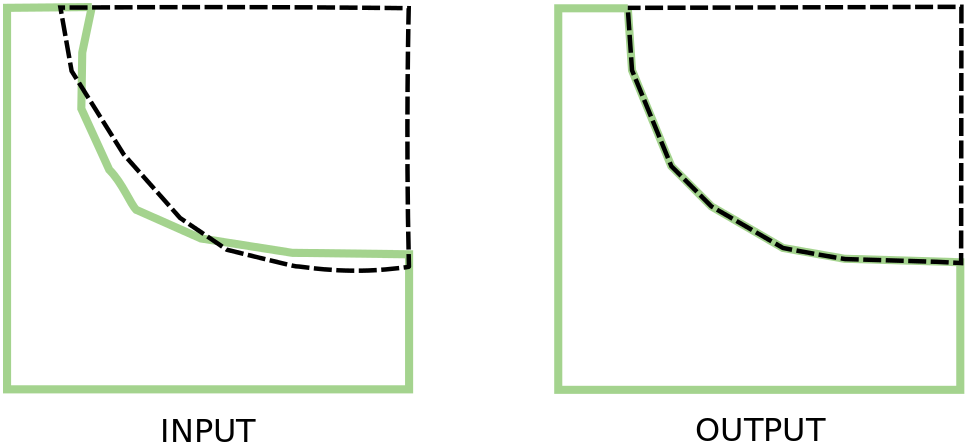
\includegraphics[width=250pt]{./pictures/integrate.png}
      \caption[Integrate - princip]{Integrate - princip 
	  (zdroj: \url{http://resources.arcgis.com/en/help/main/10.1/index.html\#//00170000002s000000})}
      \label{fig:integrate}
  \end{figure}

Nástroj \textit{Integrate} umožňuje sladění dvou datasetů. Na~vstupu vyžaduje 
dvě či více vrstev, které chceme zarovnat, a~dále maximální vzdálenost, při~které
lze považovat prvky za~odpovídající si. U~každého datasetu navíc lze zadat 
prioritu (\textit{rank}). Prvky s~nižší prioritou se pak budou zarovnávat 
k~těm s~prioritou vyšší. Tato funkce je velmi užitečná, pokud máme dvě 
překrývající se nebo sousedící vrstvy s~malými rozdíly např. v~důsledku různé
přesnosti.


\subsection{ConfleX}
\label{conflex}

ConfleX\footnote{\url{http://www.citygategis.com/conflex.htm}} 
je software pro automatické spojování vektorových \zk{GIS} dat,
který pro automatizaci využívá umělou inteligenci. ConfleX umožňuje zpracování 
i~takových případů, kdy se zdrojová mapa s~cílovou nepřekrývají nebo nejsou 
topologicky identické. Systém porovnává každé dva segmenty z~obou map a~jejich
vztah k~ostatním segmentům. Na~základě tohoto postupu pak rozhodne, zda se 
jedná o~stejné prvky či nikoli. Kromě automatického procesu umožňuje program 
i~následnou ruční editaci.

ConfleX je k~dispozici jako samostatná aplikace ale také jako extenze 
programu ArcGIS 9/10.


\subsection{Intergraph GeoMedia Fusion}
\label{geomedia}

Jedná se o~doplněk desktopové aplikace 
GeoMedia\footnote{\url{http://geospatial.intergraph.com/products/GeoMedia/Details.aspx}}
firmy Intergraph, který je dostupný od~roku 2005. Nástroj GeoMedia Fusion  
je navržen pro topologické opravy dat, validaci atributů a~integraci dat. Cílem 
je umožnit snadnou údržbu dat v~rozsáhlých geografických databázích, kde jsou 
data získávána z~různých zdrojů. Nástroj porovnává dva datasety obsahující 
rozdílné reprezentace stejné skutečnosti. Nejdříve automaticky vytvoří 
\textit{conflation links} indikující způsob spojení vrstev, které lze ještě
ručně editovat. Následně umožní geometrie i~atributy těchto dvou reprezentací
sjednotit. GeoMedia Fusion slouží k~úpravě bodových, liniových i~plošných dat
včetně jejich atributů. 


\subsection{MapMerger}
\label{mapmerger}

MapMerger\footnote{\url{http://www.mapmerger.com}} je \zk{GIS} nástroj firmy 
ESEA zaměřený na~slučování geometrie a~atributů vektorových map a~kontrolu 
kvality dat. Umožňuje převod atributů mezi dvěma překrývajícími se mapami, 
navázání hranic dvou sousedících map, přidání prvků z~jedné mapy do~druhé, 
synchronizaci mapy s~její aktualizovanou verzí, identifikaci geometrických 
a~atributových rozdílů mezi dvěma verzemi té samé mapy. První verze programu 
vyšla již v~roce 1998, od~té doby již firma vyvinula 9~verzí. Z~uvedených 
nástrojů poskytuje asi nejvíce možností zpracování a~díky specializaci 
přímo na~spojování map se řadí mezi nejvýkonnější programy v~této oblasti. 


\section{Open Source nástroje}
\label{open-source}

V~této sféře zatím neexistuje mnoho nástrojů, které by komplexně řešili problém
spojování vektorových map (\textit{conflation}). Většinou jde pouze o~malé 
programy či zásuvné moduly k~větším projektům, pomocí nichž se dá provést manuální
nebo poloautomatické sloučení vektorových datasetů, případně jejich atributů. 
Ovšem většinou je cesta k~dosažení cíle pomocí těchto nástrojů poměrně složitá 
a~ne vždy jsou výsledky takové, jak bychom si představovali. Asi jediným 
ucelenějším nástrojem je knihovna \zkratka{JCS} implementovaná jako kolekce 
zásuvných modulů v~programu OpenJUMP.


\subsection{JCS - Java Conflation Suite}
\label{jcs}

\zk{JCS}\footnote{\url{http://www.vividsolutions.com/jcs/}} je \textit{open source}
knihovna napsaná v~jazyce Java, která zahrnuje API a~soubor interaktivních nástrojů, 
které slouží ke~slučování prostorových datasetů. Byla vyvinuta společností Vivid 
Solutions, Inc. Obsahuje funkce umožňující provádění různých procesů spojených 
se~spojování vektorových map, které jsou zaměřeny především na~polygonové, případně 
liniové datasety. Co se týče bodových vrstev, je její funkcionalita poměrně omezená. 
Knihovna \zk{JCS} je závislá na~knihovně 
\zkratka{JTS}\footnote{\url{http://www.vividsolutions.com/jts/}}, která poskytuje 
základní geometrické funkce pro práci s~prostorovými daty. Obě knihovny jsou navrženy 
v~souladu s~\zk{OGC} specifikací 
\textit{Simple Features}\footnote{\url{http://www.opengeospatial.org/standards/sfs}}, 
která popisuje způsob uložení geografických digitálních dat, prostorové vztahy 
a~funkce. \zk{JCS} vznikla v~rámci projektu JUMP Unified Mapping Platform. Je 
poskytována pod~licencí 
\zkratka{LGPL}\footnote{\url{http://www.gnu.org/licenses/lgpl.html}}.

\subsubsection{Architektura}

Knihovna \zk{JCS} používá pro vizualizaci dat a~interakci JUMP WorkBench
a~API. Poskytování základní geometrické funkcionality je pak zajištěno 
knihovnou \zk{JTS}. JUMP API umožňuje vstup a~výstup prostorových dat 
a~další funkcionalitu s~nimi spojenou. Jádro \zk{JCS} tvoří Conflation API
obsahující algoritmy pro kontrolu a~slučo\-vání prostorových dat 
(\textit{conflation}). Funkce \zk{JCS} jsou v~projektu OpenJUMP 
implementovány v~podobě kolekce zásuvných modulů - \textit{QA, Conflate, 
RoadMatcher}.

  \begin{figure}[H]
    \centering
      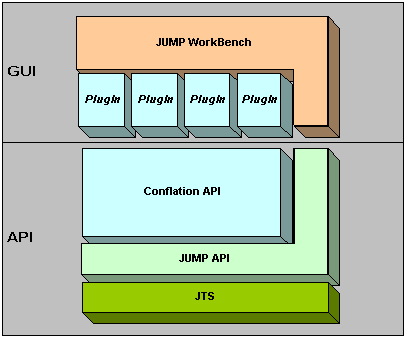
\includegraphics[width=280pt]{./pictures/JCS_Architecture.png}
      \caption[Architektura JCS]{Architektura JCS 
	  (zdroj: \url{http://www.vividsolutions.com/JCS/images/})}
      \label{fig:architektura}
  \end{figure}


\subsubsection{OpenJUMP projekt}

OpenJUMP je \textit{open source} projekt, který vyvinula firma Vivid Solutions,
Inc. Jedná se o~GIS software, který umožňuje základní práci 
s~prostorovými daty v~rastrové či vektorové podobě a~jejich atributy.

\subsubsection{JTS - Java Topology Suite}
\label{jts}

Knihovna \zk{JTS} je jedním ze~základních prvků projektu OpenJUMP.
Je napsána v~jazyce Java a~poskytována pod~licencí \zk{LGPL}. Obsahuje třídy 
pro reprezentaci geometrických objektů a~základní funkce pro práci 
s~prostorovými daty dle~specifikace \textit{Simple Features} pro \zk{SQL} 
od~\zk{OGC}. Kromě tříd reprezentujících geometrické prvky dle~zmíněné
specifikace zahrnuje další podpůrné třídy pro reprezentaci seznamu souřadnic,
aplikaci geometrického filtru (např. při~transformaci), uchovávání informace
o~maximální a~minimální souřadnici objektu a~jiné. Dále jsou součástí této 
knihovny třídy umožňující geometrické výpočty jako je vzájemná polohu bodu 
a~linie, výpočet průsečíku, prostorové analýzy, test polohy bodu a~uzavřené
oblasti atd. 

\subsubsection{Funkcionalita JCS}
\label{jcs-funkcionalita}

Projekt \zk{JCS} neumožňuje změnu souřadnicového systému. Proto se
automaticky přepokládá, že vrstvy vstupující do~zpracování mají stejný
prostorový referenční systém. Souřadnice bodů výstupních vrstev mají vždy
desetinnou přesnost.

Při většině výpočtů v~zásuvných modulech \zk{JCS} je využívána tzv. 
Hausdorffova metrika. Na~rozdíl od~euklidovské metriky totiž nezkoumá jen
nejkratší vzdálenost mezi prvky, ale i~vzdálenost největší.
Zohledňuje tedy do~jisté míry i~topologické vztahy.

Na~výpočet je Hausdorffova vzdálenost poměrně složitá. Proto se v~algoritmech
použitých v~\zk{JCS} používá spíše vrcholová Hausdorffova vzdálenost 
(\textit{Vertex Hausdorff Distance}), která není vztažena ke~geometrickému 
prvku, ale pouze k~jeho vrcholům. Tato varianta Hausdorffovy vzdálenosti 
ve~většině případů vrací stejně dobré výsledky. 

Postup spojování vektorových datasetů pomocí knihovny \zk{JCS} je založen
na~na\-le\-zení geometrických rozdílů mezi oběma mapami a~následném odstranění 
těchto rozdílů.

K~detekci geometrických odlišností je použit algoritmus pro prostorové rozdíly.
Tento algoritmus funguje tak, že postupně porovnává geometrické prvky z~obou 
datasetů, případně pouze jejich jednotlivé části, a~pokud se tyto prvky shodují,
označí je jako odpovídající si. Výsledkem jsou pak ty prvky z~obou datasetů, 
ke~kterým nebyly nalezeny žádné odpovídající prvky. Nalezení odpovídajících si
prvků probíhá následovně. Pokud je požadována přesná shoda, provede se 
testování, zda jsou prvky stejného geometrického typu a~zda se rovná jejich 
obsah. Porovnání obsahu se za\-kládá na~porovnávání jednotlivých komponent 
a~seznamu bodů daných geometrií. Ne vždy je předpokládána přesná shoda,
proto je možné určit i~prvky, které splňují podmínku danou tolerancí. Zde se
provádí porovnání Hausdorffovy vzdálenosti mezi prvky s~touto tolerancí, 
nepočítá se přitom přímo tato vzdálenost. Rozhodující je, jestliže obalová 
zóna o~velikosti vzdálenostní tolerance prvního prvku obsahuje prvek druhý 
a~naopak. Tato podmínka je ekvivalentní k~podmínce, že Hausdorffova vzdálenost
musí být menší nebo rovna toleranci. 

Pro~odstraňování překrytů či mezer neexistuje exaktní algoritmus,
ale jsou vy\-užívány různé heuristiky poskytující dobré topologické výsledky.

Následující výčet podává přehled nejčastějších úloh, které je možné 
s~tímto nástrojem řešit.

\begin{itemize}
 \item Jako \textit{Coverage Cleaning} je  označován proces hledání
    a~odstraňování topologických chyb - mezer a~překrytů v~rámci jedné
    vektorové mapy tvořené polygony či multipolygony. Detekce nežádoucích
    mezer mezi polygony je založena na~rozpoznání blízkých liniových segmentů,
    kde blízkost je určena zvolenou vzdálenostní tolerancí. 

 \item Další často řešenou úlohou je \textit{Boundary Alignment}, což by
    bylo možné přeložit do češtiny jako \uv{zarovnání či navázání hranic}. 
    Cílem je napojit k~sobě dvě vektorové vrstvy, které zobrazují sousedící
    území, tak, aby se mezi nimi nevyskytovaly nežádoucí mezery či překryty.
    Výsledkem jsou tedy plynule navazující datasety, které tvoří bezešvou mapu.
    Při této úloze je nutné zvolit přesnější referenční vrstvu, jejíž 
    geometrické vlastnosti se nezmění.

 \item U \textit{Coverage Alignment} máme na~vstupu dvě vektorové
    mapy zobrazující to samé území nebo alespoň jeho část. Tyto mapy se 
    tedy výrazně překrývají. Úkolem je upravit méně přesnou vrstvu tak,
    aby odpovídala vrstvě referenční, popřípadě její části, pokud se vrstvy
    úplně nepřekrývají. Proces spočívá v~posunutí vrcholů polygonů upravované
    vrstvy do~blízkých vrcholů vrstvy referenční.

 \item Poměrně specifickou, ale velmi častou úlohou je \textit{Road Network 
    Matching} neboli \uv{spojování silničních sítí}. Na~vstupu máme dvě 
    vektorové mapy té samé silniční sítě. Při~této úloze hledáme podobnost
    mezi liniovými prvky obou datasetů, které označíme za~odpovídající si.
    Poté je vytvořena nová vrstva silniční sítě, která obsahuje odpovídající
    si prvky, přičemž při~mírných odlišnostech použije liniové prvky z~přesnější
    mapy. \zk{JCS} bohužel zatím neumožňuje automatické provedení této
    úlohy. Pouze nalezne odpovídající si prvky a~další kroky už je nutné provést
    manuálně.

\item Úloha \textit{Geometry Difference Detection}, v~češtině \uv{detekce
    geometrických rozdílů}, na~rozdíl od~předchozích nijak neupravuje vstupní
    vrstvy ani z~nich netvoří jiné. Cílem je pouze nalézt rozdíly mezi vstupními
    datasety. Nejčastěji je používána pro rozpoznání změn mezi dvěma verzemi
    jedné vektorové mapy (např. po aktualizaci).
\end{itemize}

\subsubsection{Popis zásuvných modulů}
\label{jcs-plugin}

Zásuvné moduly ze skupiny \textit{QA - Quality Assurance} umožňují najít
geometrické rozdíly a~nesrovnalosti mezi datasety, ale také v~rámci jediného
datasetu. Funkce zde obsažené neslouží k~opravě či propojení vrstev, ale 
pouze k~identifikaci geometrických rozdílů.

\begin{itemize}
 \item \textit{Find Misaligned Segments} - slouží k~nalezení segmentů 
    ze~dvou datasetů, které by si v~rámci dané tolerance měli odpovídat,
    ale je mezi nimi mezera či překryt. 
 \item \textit{Find Overlaps} - najde překrývající se prvky ze~dvou datasetů.
 \item \textit{Find Coverage Gaps} - umožňuje nalézt mezery mezi polygony
    jednoho datasetu, které jsou užší než zadaná vzdálenostní tolerance
    a~zároveň je mezi hranami polygonů, které tvoří tuto mezeru, úhel menší
    než daná úhlová tolerance.
 \item \textit{Find Coverage Overlaps} - najde všechny překryty mezi polygony
    v~rámci jednoho datasetu, respektive všechny překrývající se polygony.
 \item \textit{Find Close Vertices} - identifikuje body (samostatné body,
    vrcholy linií či polygonů) ze~dvou různých datasetů, jejichž vzdálenost
    je menší než daná tolerance.
 \item \textit{Find Offset Boundary Corners} - slouží k~nalezení hranic
    polygonů ze~dvou sou\-sedících vektorových map, které by na~sebe měly
    navazovat, ale je mezi nimi posun menší než zadaná tolerance.
 \item \textit{DiffSegmentsPlugin} - identifikuje liniové segmenty, které
    jsou obsaženy pouze v~jedné ze~zadaných vrstev, nikoli v~obou dvou.
 \item \textit{DiffGeometryPlugin} - funguje stejně jako předchozí funkce
    s~tím rozdílem, že hledá i~samostatné geometrie (celé linie, polygony),
    nikoli jen liniové segmenty.
\end{itemize}

Další zásuvné moduly zařazené do~skupiny s~názvem \textit{Conflate} slouží
k~samotnému spojování vektorových map a~navázání dvou sousedních map.

\begin{itemize}
 \item \textit{Vertex Snapper} - identifikuje a~napojí k~sobě blízké uzlové
    body, vrcholy ze~dvou překrývajících se datasetů. Při~použití této funkce
    je nutné označit, která vrstva je referenční (s~body z~této vrstvy se 
    nebude hýbat).
 \item \textit{Coverage Alignment} - zarovná geometrii jednoho datasetu 
    k~jinému referenčnímu datasetu v~místech, kde se překrývají nebo spolu
    sousedí. Na~rozdíl od~předchozí funkce nepracuje pouze s~odpovídajícími
    si body, ale s~celými geometriemi.
 \item \textit{PolygonToolboxMatcherPlugin} - tento nástroj slouží k~identifikaci
    podobných polygonů ve~dvou různých datasetech, přičemž umožňuje různá 
    nastavení tak, aby bylo možné najít opravdu jen odpovídající si polygony
    popřípadě více polygonů odpovídajících jednomu či naopak. 
 \item \textit{AlignmentToolboxPlugin} - slouží k~zarovnání dvou vrstev k~sobě.
    Bohužel zatím není plně funkční.
\end{itemize}

Skupina označena jako \textit{Clean} obsahuje funkce k~k~opravě nepřesností
nalezených pomocí funkcí skupiny \textit{QA} v~rámci jednoho datasetu.

\begin{itemize}
 \item \textit{Remove Coverage Gaps} - odstraní mezery mezi polygony jedné
    vrstvy dle~zadané tolerance.
 \item \textit{Remove Short Segments} - tato funkce by měla dokázat odstranit
    liniové segmenty kratší než daná tolerance tak, aby co nejméně porušila 
    topologii vrstvy. Zatím však umožňuje pouze odstranění krátkých izolovaných
    segmentů.
 \item \textit{CoverageCleaningToolboxPlugin} - poskytuje stejnou funkcionalitu
    jako první ná\-stroj z~této skupiny, navíc umožňuje odhalit překryty 
    mezi polygony jedné vrstvy.
\end{itemize}

Poslední skupina zásuvných modulů je nazvána \textit{Roads}. Zabývá se 
spojováním vektorových map silniční sítě.

\begin{itemize}
 \item \textit{RoadMatcherToolboxPlugin} - umožňuje vytvořit vrstvu s~rozdíly
    mezi silnicemi ze~dvou vrstev a~na~základě těchto rozdílů a~identifikovaných
    společných prvků jednu z~těchto vrstev navázat na~druhou referenční tak, 
    aby si odpovídaly.
\end{itemize}


\subsection{OpenStreetMap}
\label{OSM}

OpenStreetMap je projekt sloužící k~tvorbě a~vizualizaci geografických dat.
Jedná se o~\textit{open source} projekt, což znamená, že ho může kdokoli 
využívat a~přispívat do něj. V~OpenStreetMap existuje mnoho nástrojů 
pro editaci prostorových dat a~některé z~nich umožňují i~manuální nebo
poloautomatické spojování datasetů z~různých zdrojů (\textit{conflation}). 
Bohužel ani zde však neexistuje žádný komplexnější nástroj jako je výše
popsaná \zk{JCS}. Navíc většina těchto nástrojů je vytvořena pro nějaký
konkrétní účel jako např. pro spojování silničních sítí v~USA a~ne vždy
je proto jejich použití zcela obecné. Uživatel si tedy mnohdy musí poradit
sám a~použít několik různých nástrojů, aby dosáhl požadovaného výsledku.
Dále uvádím nástroje, které lze pro některé činnosti související 
se~spojováním map použít. 

\subsubsection{JOSM conflation plugin}

\zkratka{JOSM} je desktopová aplikace umožnující
editaci dat projektu OpenStreetMap. Jedním ze~zásuvných modulů pro tuto 
aplikaci je \textit{Conflation}, který umožňuje spojování vektorových dat. 
Tento nástroj však je stále označen jako experimentální, což znamená, že ne 
vždy funguje zcela správně. Nástroj umožňuje zarovnat prvky jedné vrstvy tak,
aby souhlasily s~prvky druhé vrstvy, která je označena za~referenční. 

  \begin{figure}[hbt]
    \centering
      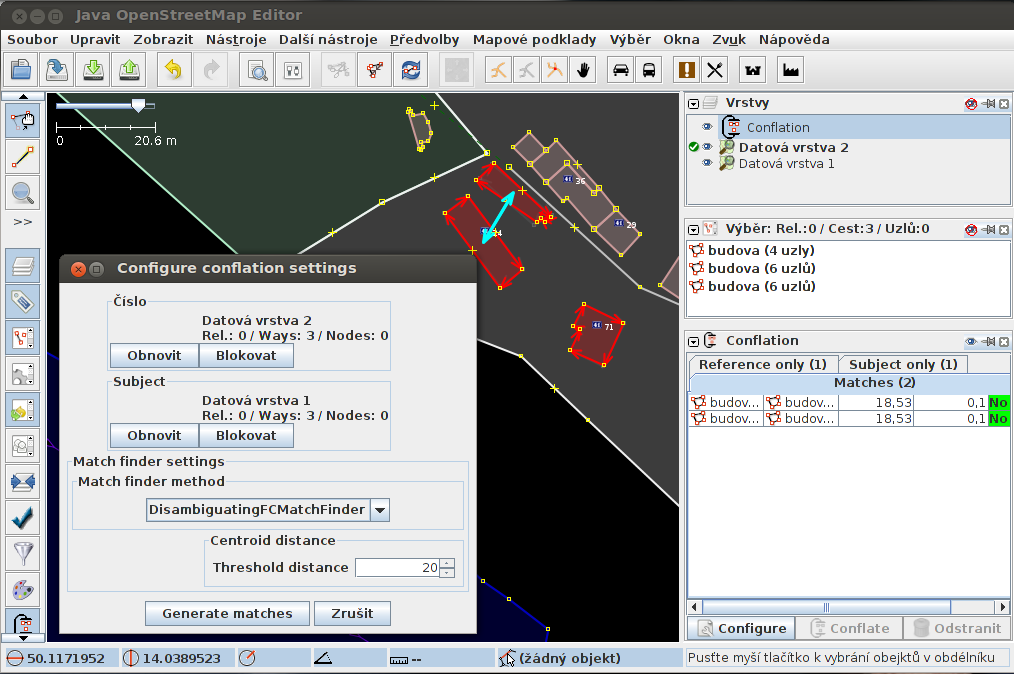
\includegraphics[width=280pt]{./pictures/josm.png}
      \caption{JOSM conflation}
      \label{fig:josm}
  \end{figure} 

V~prvním kroku je určena referenční a~upravovaná vrstva. Poté je třeba v~obou
těchto vrstvách označit prvky, které by si měly odpovídat. V~dalším kroku se 
provede automatická identifikace dvojic vybraných prvků z~obou datasetů 
a~nakonec se vykoná samotný proces zarovnání prvků (\textit{conflate}), kdy 
jsou prvky upravované vrstvy změněny tak, aby odpovídaly prvkům vrtsvy 
referenční. Jedná se o~proces poloautomatický, jelikož nejdříve je třeba
ručně identifikovat odpovídající si prvky a~teprve na~základě tohoto kroku je 
provedena automatická úprava prvků.

\subsubsection{Potlatch 2 merging tool}

\textit{Potlatch 2 merging tool} je nástroj původně navržený pro spojování 
vektorových dat cyklistických tras v~rámci England Cycling Data 
Project\footnote{Projekt pod záštitou britského ministerstva dopravy, 
který si klade za~cíl umožnit dostupnost informací o~síti cyklostezek
ve~Velké Británii prostřednictvím OpenStreetMap.}. 
V~případě tohoto nástroje se jedná především o~proces přenosu atributů. 
Pokud máme v~mapě dva odpovídající si prvky, pomocí tohoto nástroje je 
můžeme označit za~odpovídající a~jednoduše sloučit jejich atributy. Nutno 
však podotknout, že výběr odpovídajících si prvků musíme provést vždy ručně. 


\subsection{Univerzitní projekty}
\label{univerzitní}

Mimo výše uvedené nástroje existuje také několik projektů různých světových
univerzit zabývajících se buď kombinací geo\-grafických dat obecně nebo 
spojováním map silničních sítí. Možnosti využití těchto programů pro běžného
uživatele se velmi různí. A~ne vždy lze zcela volně tyto nástroje vyzkoušet. 
Jedním z~nich je i~Conflation System MBP, který byl vyvinut na~katedře počítačů 
(\textit{Computer Science Department}) na~Central Washington University v~USA. 
V~rámci tohoto projektu vznikl \textit{MBPConflate} software, který má přispět 
k~výzkumu v~oblasti slučování geo\-grafických dat. Program umožňuje automatické 
spojení map, poskytuje nástroje pro následnou kontrolu kvali\-ty výsledné mapy. 
Je navržen tak, aby bylo snadné implementovat nové techniky a~algoritmy v~této 
oblasti. Bohužel se mi k~tomuto nástroji nepodařilo najít iformace o~licenci. 

   \begin{figure}[hbt]
     \centering
       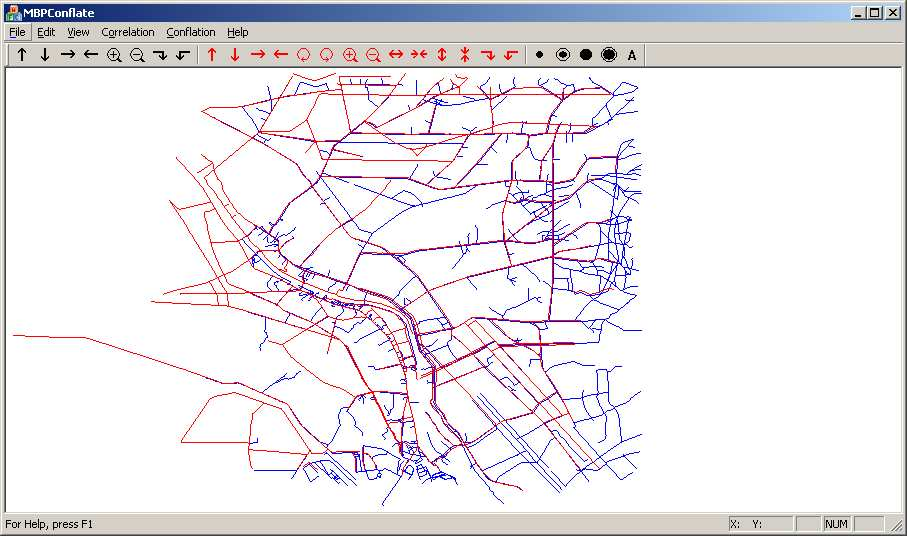
\includegraphics[width=280pt]{./pictures/MBPconflate.png}
       \caption[MBPConflate]{MBPConflate (zdroj: \cite{mbp})}
       \label{fig:mbp}
   \end{figure}

\cleardoublepage\chapter{Zatím nevím}
\label{4-nevim}

\section{GEOS - Geometry Engine, Open Source}
\label{geos}

\textit{GEOS (Geometry Engine - Open Source)} je knihovna implementující 2D prostorové predikáty a funkce dle~OGC specifikace \textit{Simple Features} pro SQL. \textit{GEOS}
je přepisem knihovny \textit{Java Topology Suite (JTS)}, o~níž jsem se zmiňovala výše, do~jazyka C++. Knihovna je projektem OSGeo (The Open Source Geospatial Foundation) a je
dostupná pod licencí LGPL.

\section{OGR Simple Feature Library}
\label{ogr}

\textit{OGR Simple Feature Library} je \textit{open source} knihovna umožňující čtení a poř. i zápis vektorových dat různých formátů jako je ESRI Shapefile, S-57, SDTS, 
PostGIS, Oracle Spatial atd. \textit{OGR} je součástí knihovny \textit{GDAL}\footnote{Geospatial Data Abstraction Library - knihovna umožňující čtení a zápis rastrových dat}.

\section{Quantum GIS}
\label{qgis}

\textit{Quantum GIS} je \textit{open source} geografický informační nástroj, který patří mezi~oficiální projekty \textit{Open Source Geospatial Foundation} 
(OSGeo)\footnote{http://www.osgeo.org/}. QGIS je napsán v~jazyce C/C++, je publikován pod~licencí \textit{GNU General Public License}\footnote{http://www.gnu.org/licenses/gpl.html}
a~je multiplatformní. Program umožňuje zpracování a~analýzy vektorových i~rastrových dat. Kromě základní funkcionality, která je zajištěna samotnou aplikací, existuje ještě 
velké množství volně dostupných zásuvných modulů psaných v~jazycích C++ a~Python umožňujících poměrně široké využití tohoto nástroje.

QGIS začal vznikat v~roce 2002. Původní myšlenka vzešla z~potřeby prohlížeče GIS dat pro~Linux, který by podporoval většinu existujících formátů. To vedlo k~vytvoření 
\textit{Quantum GIS} projektu. Úplně první verze podporovala pouze \textit{PostGIS}\footnote{prostorová nadstavba databázového systému \textit{PostgreSQL}} vrstvy, poměrně 
rychle však byla doplněna podpora i~dalších datových formátů a~QGIS se z~pouhého prohlížecího nástroje stal plnohodnotným geografickým informačním systémem.


\subsection{Zásuvné moduly}
\label{qgis plugins}
...


%**************************************************************

%\bibliographystyle{abbrv}
%\bibliography{literatura}

\appendix

%\cleardoublepage\include{priloha-prirucka}

\end{document}
